\chapter{all intros}
\section{ultimate conductivity}
The unique behaviour displayed by nanoscale-sized materials is responsible for numerous scientific and technological breakthroughs. In comparison to their bulk counterparts, nanomaterials often reveal superior physical properties. Nonetheless, despite the unprecedented level of control that is currently possible over their structure, the manipulation of individual nanoscale components is still extremely laborious. For this reason, industry and academia have sought to exploit these functionalities without the need for precise nanomaterial placement. Candidates of particular interest are films comprised of randomly dispersed nanowires, commonly known as nanowire networks (NWNs).

NWNs are promising alternatives for a wide range of applications including flexible transparent conductors,1-3 thin-film solar cells,4 field-effect phototransistor5 and sensor6 devices, to name but a few. Formed by randomly dispersed conducting wires, NWNs may function as conducting materials depending on the degree of connectivity of the network as well as on the quality of the junctions formed between neighbouring wires. Effective signal transmission through the wires depends on the nature of coating layers or surface functionalization on these wires. Because these coatings are typically dielectric in nature, NWNs can be thought of as an array of randomly dispersed conducting wires connected by capacitive junctions which will only conduct current if the voltage drop across a junction exceeds its characteristic threshold voltage.7 Once this occurs, charge flows across the network through percolative paths formed by wires connected by resistive junctions.

The conduction properties of NWNs is dictated by a multitude of parameters such as the wire length and diameter distribution,8 interwire contact resistance, inner-wire resistance, wire density as well as their connectivity profile. With so many possible variables, such a study is best carried out through computer simulations. One way of simulating this percolative transport problem9,10 is to map the network into a node voltage problem: each wire is represented by a circuit node at a common voltage connected to other wires by a certain number of junction resistances that depends on its connectivity within the network. Within this representation, it is then straightforward to obtain the overall conductance of a network by merely applying Ohm's and Kirchhoff's current laws.11,12 However, this approach involves an implicit assumption, hereafter referred to as the junction-dominated assumption (JDA), that the most significant contribution to the overall conductivity comes exclusively from the interwire junction resistances. This assumption is the basis for most earlier descriptions of NWNs, including a recent theoretical calculation to describe the sheet resistance and the optical transmittance of Ag NWNs13 where the characteristic junction resistance was then adjusted to match available experimental data.11

The JDA is perfectly safe when the junction resistance is significantly larger than any other characteristic resistances within the network. This indeed is the case of NWNs comprised of carbon nanotubes.14,15 However, the demands for increasingly conductive films, driven by efforts to reduce the junction resistances, will ultimately undermine the validity of the JDA due to its neglect of the inner resistances of the wires.16 By relaxing the JDA, we can account not only for the geometric aspects of the network but also for the material properties of its components. Furthermore, by extending this picture to the limit of vanishingly small junction resistances we can provide an upper bound for the conductivity of the NWNs and reveal how much room there is to improve the conductivity of a film. Rather than working with computer-generated random networks, it is desirable to establish the upper bound for the conductivity of real networks. When conductivity measurements of such networks are compared with their respective upper bounds, one has a clear indication of how close to the optimum value they are. This calls for a computational tool capable of capturing the geometry of real networks combined with the ability to calculate the sheet resistance of the corresponding array of inter- and inner-wire resistors.

In this manuscript, in addition to relaxing the JDA as described above, we present for the first time a set of simulations that obtain the sheet resistance of networks with defined geometries through SEM image analysis of real samples (cf.Fig. 1). In this way, we have a one-to-one correspondence between simulation and experiment and can simulate both the actual and ultimate network conductivity, the latter assuming the junction can be further optimized. Networks to be simulated were built from real experimental images of sparse and dense samples with wire densities (n) ranging from 0.15-0.6 wires per μm2. This approach avoids the need for spatial configurational averaging highlighted in a recent paper in reference 12. Instead, our simulated network captures exactly the same spatial arrangement of the network displayed on the SEM images. The inner-wire resistance was included using a novel node-voltage approach capable of describing the transport properties of NWNs that also accounts for the wires resistivity. The model uses a new mapping scheme in which the wires of the network are described by a multi-nodal representation (MNR); the network topology is mapped as a graph carrying information about the wire junction connections and their respective separations. Critically, the model outputs for each network a set of characteristic values that are determined by the network connectivity and that allow a direct comparison between distinct networks. Such explicit examination of NWNs would not be possible throughout traditional configurational averaging approaches.
%-----------------------------------
\section{Transfer}
Nano-scale level control in material science has lead to unprecedented technological advances in recent years. Nano-scale devices are seeing application in a broad range of fields, from computer chips to bio-medical devices. Creating structures at increasingly minuscule resolutions has proved to be challenging, costly and, difficult to scale for industrial application. Naturally there is a demand for nano-scale devices that can be fabricated at a low cost and in great volume while still retaining their desirable properties.

One such material that fulfills these conditions are thin films composed of randomly dispersed nano-wires, known as Nano-wire Networks (NWNs). A Scanning Electron Micrscope (SEM) image of a typical NWN can be seen in Fig.\ref{fig:nwn_image}. 
\begin{figure}[ht!]
\centering
\includegraphics[width=0.4 \columnwidth]{4_C5_crop.png}
\caption{\fontsize{10pt}{9pt}\selectfont \textit{SEM image of a typical NWN. Electrodes can be seen on either side of the NWN. The size of this sample is approximately $20 \times 20 \mu m^2$}}
\label{fig:nwn_image}
\end{figure}
NWNs have a relatively simple, cheap and, easily scalable fabrication processes such as spray coating\cite{rocha2015}, drop casting\cite{hardin2011} and, spin coating\cite{leem2011}. Each technique has its merits but spray coating in particular leads to a very homogeneous network, is scalable and can be performed under normal atmospheric conditions \cite{langley2013}. Tenent et al\cite{tenent2009} used spray deposition to fabricate networks of randomly arranged Carbon Nanotubes of size of $6 \text{inches} \times 6 \text{inches}$ demonstrating that large devices can be made.

Thin films that couple high electrical conductivity and optical transparency are crucial in a number of applications such as touch screens, solar cells and liquid-crystal displays. There is much interest in transparent conductive materials (TCs) that are also highly flexible in order to create materials such as electronic paper and foldable displays. NWNs have displayed excellent optoelectric and mechanical properties which makes them a strong candidate for creating flexible TCs. As such NWNs made from a number of materials have been used to create TCs \cite{madaria2010, sakunta2009,sukanta2011}. 

\begin{figure}[ht!]
\centering
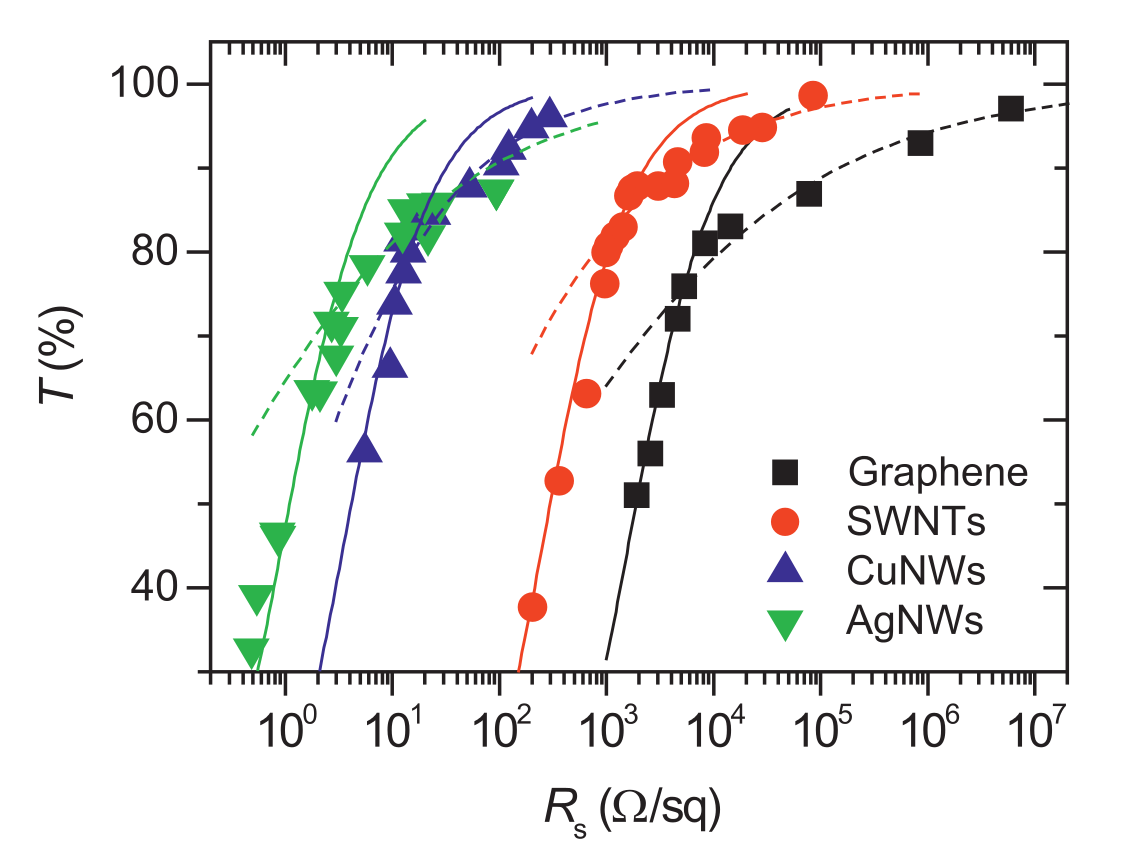
\includegraphics[width=0.6 \columnwidth]{trans_res_diffMat.png}
\caption{\fontsize{10pt}{9pt}\selectfont \textit{The transmittance of a number of different TC's made from different materials was compared with their respective sheet resistance by De et al\cite{sukanta2011}. Points are fit to expressions describing the percolation regime (dashed line), or low wire density regime, and the bulk regime (solid line).}}
\label{fig:opt_prop}
\end{figure}
A wide range of TCs were compared by De et al\cite{sukanta2011}. Shown in Fig.\ref{fig:opt_prop} is a comparison of optical transmission for a given sheet resistance for Graphene networks, silver NWNs, copper NWNs and, single walled carbon nanotube networks. TCs require low sheet resistances and high optical transmission ($T \geq 90\%$). As shown in Fig.\ref{fig:opt_prop} this typically occurs in low wire density NWNs. 

Sheet resistance is used as a measure of resistance of thin films. Given a thin film, as in Fig.\ref{fig:sh_res}, of thickness $t$, width of $W$, distance between electrodes is $L$, and resistivity $\rho$. If electrodes were applied to the two opposite $tW$ faces, the resistance between them is
\begin{equation}
R = \frac{\rho L}{W t} = R_s \frac{L}{W}
\end{equation}
Where the sheet resistance $R_s = \frac{\rho}{t}$.

\begin{figure}[ht!]
\centering
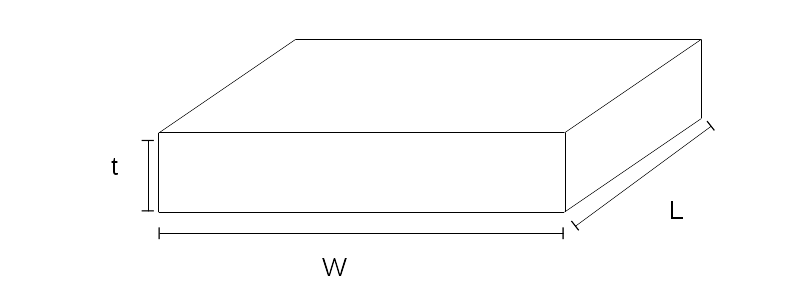
\includegraphics[width=0.6 \columnwidth]{sheet_res.png}
\caption{\fontsize{10pt}{9pt}\selectfont \textit{A sketch of a thin film of thickness $t$, width $W$ and length $L$. The electrodes are applied at on the $Wt$ faces.}}
\label{fig:sh_res}
\end{figure}

It has been shown by Madaria et al that Silver NWNs can remain conductive when bent up to 160 degrees and returned to their original sheet resistance when the bending stress was removed \cite{madaria2010}. Lim et al \cite{lim2012} examined various mechanical properties of Ag NWNs. NWNs were bent, twisted and put under torsional stress. Samples were bent several thousands of times with no significant change in the sheet resistance. Samples were twisted up to an angle of 40 degrees with a $~0.5\%$ change in sheet resistance. Samples were stretched up to $4\%$ their original length a change of $~0.4\%$ in sheet resistance. The flexibility of NWNs coupled with their excellent optoelectrical properties make them a promising material for flexible TCs. 

The electrical properties of NWNs are known to depend on a number of parameters. Hecht et al reported the dc conductivity scaled with the average length of Carbon Nano-tubes ($L_{av}$) as $~L_{av}^{1.46}$\cite{hecht2006}. We have shown in simulations how the resistivity of a material can add greatly to the sheet resistance of the NWN\cite{rocha2015}. A number of authors have reported that the electrical and optical properties depend on the wire density in the NWN\cite{mutiso2013,tenent2009,hecht2011}. Fairfield et al have shown the sheet resistance depends on the shape of the electrode used to contact the network\cite{fairfield2014}. 

In order to understand how the sheet resistance depends on these physical parameters some theoretical framework must be used. In Fig.\ref{fig:nwn_image} one can see the sheer complexity involved, where junction resistance, wire lengths and, wire widths follow distributions and wires have random spatial arrangements. Thankfully Kirchhoff's circuit and Ohm's laws can be used to describe resistive networks using a system of linear equations (this method is explained further in a later section).

There is a downside related to this method however. This method does not result in a functional form for the sheet resistance. One must perform fits to the results of simulations in order to determine dependencies of certain parameters. Also, due to the vast complexity of the system mentioned above, simulations must be averaged over a large number of samples in order extract average results. This results in computationally expensive simulations which in turn limits the size of NWNs that can be examined. Simulations are confined to networks with less than 15,000 wire junctions (this corresponds to a NWN of wire density 0.5 and size $45 \mu m^2$). In order to reduce the complexity and to allow us to compare simulations with experiment more directly we developed a method to record the spatial properties of a network\cite{rocha2015}, i.e the positions of wires and the points of intersections of wires. This work is presented in following sections.  

Percolation theory has been applied two dimensional stick systems for the past four decades. This is a natural framework to use in order to explain the properties of NWNs. Percolation theory is a method to describe the flow of a physical parameter (such as electrical current or water) through a random network. Pike and Seagar used percolation theory to describe a critical density of 2D randomly oriented sticks ($(n_w)_c$) of length $l$ where in a system with a wire density less than this no conducting paths would form between the electrodes\cite{pike1974}. The expression for this is given in Eq.(\ref{perc})
\begin{equation}
(n_w)_c l^2 = Q
\label{perc}
\end{equation}
Where Q was found to be 5.71. By fitting simulation data to a semi-empirical model Li and Zhang found a more precise value recently and give $Q = 5.63726 \pm 0.00002$\cite{li2009}.

Percolation theory has also been used to study how the sheet conductance $g$ depends on the wire density $n_w$. Percolation theory suggests the relationship:
\begin{equation}
g \propto (n_w - (n_w)_c)^t
\end{equation}
For wire densities in the criticality region, where $n_w \approx (n_w)_c$, Li and Zhang have shown $t\approx 1.280 \pm 0.014$. For wires densities beyond the criticality region, Li and Zhang have shown that the conductivity exponent $t$ depends on both the junction resistance $R_j$ and the intra-wire resistance $R_i = \rho l$ where l is the length of each wire in the system, and $\rho$ is the resistivity per unit cross sectional area\cite{li2010}. They found that $t$ could be described well through fitting an error function
\begin{equation}
t(x) = t_0 + A~ Erf(x), ~~ x = log_{10}\left(\frac{R_j}{R_i}\right)
\label{perc_exponent}
\end{equation}
where $t_0$ and $A$ are fitting parameters of values $1.314 \pm 0.002, ~ 0.108 \pm 0.003$ respectively. $Erf(x)$ is the error function. Eq.(\ref{perc_exponent}) tested for values in the range $-6<\log_{10}(R_j/R_i)<6$. Li and Zhang's simulations suggest that t lies in the range $1.206 \leq t \leq 1.422$. 

Percolation theory suggests functional forms to describe the scaling of the electrical behaviour. Li and Zhangs work shows that the this depends on wire length, wire density, junction and, intra-wire resistances. However these dependencies were obtained through the use of fitting semi-empirical functions to computational and physical experiments. It would be much more desirable to have a closed form expression that requires no such fitting of functions. Our work towards a closed form expression is presented later.

In order to describe NWNs we will approximate them using regular and periodic resistive lattices, on which much work has been done. Cserti\cite{cserti2000} considered a regular, periodic infinite resistive networks and derived a closed form expression that gives the resistance between any two nodes in the network. In 1973 Kirkpatrick\cite{kirkpatrick1973} presented an effective medium theory (EMT) to describe a network with a random distribution of conductances. This involves calculating an effective conductance such that when every conductor in the network is replaced with this conductance, the overall sheet conductance is the same as that when the conductors follow the distribution. We propose a combination of lattice resistive Green's functions and Kirkpatrick's EMT can be used to approximate the sheet resistance of NWNs and provide an understanding of how the sheet resistance depends on physical parameters outlined above.

In later sections we present methods to describe the electrical properties of NWNs where intra-wire resistance is neglected and when it is not. For silver NWNs typical intra-wire resistances lie in the range $3-9 \Omega$ for wire densities in the range $~0.2-0.6 \mu m^{-2}$. This compares with the average junction resistance of $~11 \Omega$. This suggests that intra-wire resistance should play a large role on the sheet resistance of NWNs. A method that incorporates the intra-wire resistance has never before been implemented. This will then be used to show the sizeable effect the intra-wire resistance in Ag NWNs can have. Following this a derivation that describes the sheet resistance of finite sized regular resistive networks of any type is presented for the first time. This is then successfully coupled with an EMT that we tailored to NWNs to provide an analytical expression describing the electrical properties of NWNs.  
%-----------------------------------
\section{EMT}

Randomly dispersed nanowires networks (NWN) are flexible, electrically active materials with great promise for use as transparent conductors \cite{liang2014,bergin2012,langley2013}, thin-film solar cells \cite{song2013,dechan2015,kim2013}, and sensor devices \cite{choi2008,datta2014}.  NWNs are most typically comprised of metallic nanowires, of which each wire is coated with either a surface functionalisation or oxide passivation layer to facilitate solution phase processing by preventing flocculation. The exploitation of NWNs for any of these applications involves the activation or switching on of the junctions between wires in the network, which is typically accomplished by using heat\cite{madaria2010,hwang2014}, pressure\cite{liangbing2010} and electrical stressing\cite{nirmalraj2012} to yield a material with definitive properties, e.g., sheet resistance and transparency.

Fig. \ref{fig:image}(a) shows an SEM image of a typical NWN, where hundreds of high aspect-ratio wires are randomly deposited onto an insulating substrate and contacted by two metallic electrodes on opposite ends of the image. Whilst such NWN devices may require no precise spatial ordering, accurately predicting the physical responses of such a system is challenging due to the large uncertainties caused by two main types of disorder: the randomness with which wires are spatially distributed and the inherent fluctuations on the individual characteristics of the wires. This calls for averaging strategies that reduce the impact of these fluctuations in any calculations. With that in mind, we have recently introduced a method that processes SEM microscopy images of NWNs and captures the precise locations of all wires of a given sample\cite{rocha2015}. This establishes the exact connectivity the NWN possesses and removes the need for averaging over the wire locations, consequently reducing the fluctuations induced by spatial disorder. 
 \begin{figure}[h!]
\centering
\includegraphics[width=0.7\columnwidth]{nwn_network_sketch.jpg}
\caption{(a) SEM micrograph image of a Ag-NWN with hundreds of wires randomly distributed on top of an insulating substrate. Two electrodes on both sides of the sample, shown as vertical gray bars, are connected by numerous paths formed by the wires. (b) After the image is processed, the digitized version of the image records each wire location and provides full information about the intersection points of each wire; (c) Mathematical graph showing voltage nodes as points and connecting resistors as edges; (d)  
The simplified graph of a square lattice representing a regular ordered network. }
\label{fig:image}
\end{figure}

This image-processing technique is a welcome tool to improve the descriptive power of simulations but the study of the electrical response of these films remains challenging because it also depends on a multitude of other factors such as material type, wire length and diameter, interwire contact quality, wire density, network connectivity, etc. It is frequently assumed to facilitate calculations of this type that the overall network resistance is dominated by the junction resistances formed between adjacent wires of the network\cite{mutiso2013}.  However, calculated junction resistances based on this assumption have now been shown to be orders of magnitude higher than those subsequently measured\cite{bellew2015}, indicating that the internal contribution of the individual nanowires cannot be neglected and is one more factor to be accounted for. With so many ingredients affecting the sheet resistance of these films, a closed-form expression for the conductance of such heavily disordered networks would be very welcome. 

At present, there is no theoretical description based on real-world NWNs in which their far-from-perfect physical characteristics are accounted for in a closed-form mathematical representation. This is typically done by means of laborious Monte-Carlo procedures used to determine universal behaviours of simplified computer-generated NWNs  \cite{pike1974,li2009,zezelj2012,ashkan2007}. Indeed, such techniques are so computationally demanding that the dependence of the sheet resistance on all the possible physical characteristics of real NWN such as the wire density, material properties, connectivity, etc, can only be estimated numerically. However, closed-form analytical expressions for the conductance of ordered homogeneous networks are known \cite{cserti2000}. These are spatially ordered networks ({\it e.g.}  square, triangular, hexagonal, etc) connected by identical resistors throughout. Whether these expressions can be of use to describe heavily disordered structures, even though they are far from ordered and homogenous, is the question posed here. In this manuscript we show that by mapping the disordered structures onto a corresponding effective medium, we can obtain the sheet resistance of NWN with an arbitrarily large density of wires. Further manipulation of these expressions enables us to describe the conductivity of these films under real experimental conditions. In fact, we show that dense networks composed of nanowires of non-uniform lengths and diameters contacted by finite-sized electrodes can be fully described by this approach. Furthermore, we argue that not only can we reproduce experimental measurements but we are also able to search for optimization conditions that will minimize the sheet resistance of a NWN.
 
The sequence adopted in this paper is as follows. For the sake of completeness, we start by writing the equivalent resistance (or conductance) of a network comprised of identical resistors forming an infinitely large regular ordered lattice. Because Kirchhoff's laws on networks are expressed in terms of a Laplacian matrix, it is useful to solve this problem using Green Function (GF) methods. Indeed, writing it in terms of GF becomes extremely convenient when disorder is included since there is a vast body of knowledge on solving Laplacian-like equations\cite{cserti2000} for disordered matrices\cite{economou1984, pingsheng}. We then present the effective medium theory (EMT) that allows us to express the problem of calculating the conductance of a inhomogeneous disordered network in terms of an ordered regular network that has a homogeneous resistance\cite{kirkpatrick1973}. Without any fitting parameter, we are able to demonstrate that this closed-form expression for the conductance provides an excellent match both with simulations and with experimental results. We conclude by illustrating how this approach can be useful in the study of NWNs as well as in other disordered materials. 
%-----------------------------------
\section{Co-percolation}
Metallic nanowire networks are flexible, electrically active materials with great promise for use as transparent conductors,1-3 solar cells,4-6 fuel cells,7-9 generators,10 stretchable11-15 and sensing16,17 devices. These networks typically consist of randomly dispersed metallic nanowires coated with an active dielectric shell, either as the result of oxidation or due to passivation chemistry necessary to prevent flocculation in solution. The presence of this outer shell results in the emergence of new and intriguing electronic properties. For example, networks made of polymer-coated silver nanowires with high aspect ratio and modified junction resistance are known to produce the lowest sheet resistances,1,17-22 whereas oxide-coated nickel nanowire networks demonstrate electrically-induced programmability.23 Nanowire networks comprised of either material act as memristive systems whose sheet resistance (Rs) depends on the electrical measurement history of the network,24 stemming from the collective response of nanowire-nanowire junctions that serve as memristive units.

In these electrically stressed networks, it is critical to control the activation voltage of the sample (Von), a threshold voltage at which a conducting percolative path is formed across the network and current can begin to flow through the material. The reduction of Von is an important challenge, especially for large area networks whose memristive response can only be activated by extremely high voltages. For instance, square Ni nanowire networks with lateral dimensions (d) ranging from 100-200 μm can require activation voltage values ranging from 100-200 V.18 We have previously shown an efficient strategy to tune activation voltages and sheet resistances of nanowire network materials by altering the shape of the electrodes, which lowers Von and the network sheet resistance by over 40%.25 The conducting features of nanowire networks can also be controlled using a wide range of experimental procedures such as application of heat,2,3,26 light,27,28 or compression,29 however many of these approaches remove the evolutionary behavior required to create programmable materials and neuromorphic circuits.30 New approaches are needed that do not sacrifice the characteristic synthetic memory of nanowire networks, to enable larger networks to manifest memristive response at low voltages.

Here we show that synthesizing heterogeneous nanowire networks composed of a mix of Ag and Ni nanowires is an effective strategy for controlling the voltage needed for both activation and the onset of memristive hysteresis loops. We demonstrate that relatively small percentages of Ag nanowires are needed to effectively tune the conducting features of the samples, even in sparse networks. Simulations support this observation and show that heterogeneous Ni/Ag networks are electrically activated at a considerably lower voltage than pure Ni networks. However, above a certain density threshold the addition of Ag nanowires saturates the system, resulting in a percolative silver network in which current bypasses the Ni nanowires. Remarkably, sufficiently large area Ni/Ag networks could be electrically activated and demonstrated memristive behaviors which are normally not achieved for Ni-only networks of same sizes. While co-percolation31 has been previously demonstrated in conducting films of Ag nanowires and carbon nanotubes,32-34 this is the first demonstration of a co-percolating nickel and silver network, and the first co-percolating network to demonstrate resistive switching. By expanding our previous computational network model25 to include dynamical activation, we also demonstrate the importance of Ag nanowires in controlling and modifying local current connectivity. Our fabrication method for co-percolating networks is considerably simpler to implement than competing hybrid networks with layers of different metals which require many processing steps for synthesis or fabrication.35,36 These results enable efficient use of noble metal nanowires, by showing that the electrical performance of Ni nanowire networks can be dramatically improved by adding small amounts of expensive Ag nanowires, while retaining memristive behavior needed for smart sensing and neuromorphic computation.
%-----------------------------------
\section{Scaling}
The unique properties of nanoscale materials are well established and they have been responsible for numerous scientific and technological breakthroughs in last decades. In comparison to their bulk counterparts, nanomaterials often reveal superior physical properties such as higher strength, lighter weight, increased electrical conduction, and greater chemical reactivity. Currently, these properties are exploited through the integration of individual components (dots, wires, sheets) into devices or from the benefits derived from the assembly of these components into networks and composites. In each case the presence of surface layers -molecules, surfactants, polymers and native oxides - essential to stabilize these materials during synthesis and processing, represent barriers to physical integration and electrical connectivity. Thermal, mechanical and chemical processes have been employed to minimize these barriers and develop various applications based on metal nanowire networks (NWN) [1, 2] including flexible and transparent conductors [3, 4, 5, 6, 7, 8, 9, 10], energy storage [11, 12] and generator devices [13,14, 15], sensors and memory devices [16, 17]. Nanoscale dielectric layers give rise to material-independent ubiquitous behaviors. For example, electrical stressing of junctions between oxide coated wires show resistive switching; polymer coated wires undergo controlled capacitive breakdown, whereas wires coated with semiconducting layers exhibit memristive-like properties [18, 19, 20, 21, 22, 23, 24] in which their electrical resistance depends on the history of the applied current or voltage drop. Identical behaviors are found in planar metal-insulator-metal structures [25, 26, 27], despite the different geometry and vastly different contact areas. A single metal-insulator-metal memristive structure manifests complex non-equilibrium dynamics that are central for the development of next-generation memory devices and brain-inspired technology. These field-driven behaviors are pervasive on the nanoscale and have led to speculation about the formation of single "winner-takes-all" (WTA) conducting filaments (CF) that are believed to dominate conduction and memory performance [25, 28]. Note that in the context ofIn the case of artificial neural networks, WTA networks are algorithms in which neurons in a layer (mostly the output) compete with each other for activation until only one neuron wins and becomes active, namely the one associated to the strongest input signal [29, 30, 31]. Here the WTA scenario is addressed in ahas a physical solid-state context representation in which mobile ions in the metal- insulator-metal junction start to cluster in response to the applied electric field, with the largest cluster growing more rapidly than others [32, 33]. Once the first CF is formed, conduction in the channel is established hindering hence the growth of any subsequent filaments.

Here we demonstrate that it is possible to form WTA connectivity paths in macroscale nanowire networks. The existence of WTA paths is critical to establishing independently addressable memory or conductance states in complex systems. We describe the network properties necessary to establish a WTA path and the possibility of addressing nanoscale components within a macroscopic assembly without the need for direct contacts. To demonstrate this capacity, we first explore the relationship between the electrical behaviors of junctions formed between individual nanowires (NWs), with those of macroscopic assemblies of the same junctions present in  random NWNs. We find that for both the increase in conductance scales identically with the current compliance limit used to assess the I-V characteristics of the system. This self-similar scaling holds for all nanomaterial systems studied and simulations reveal it is a property of any network where the junctions dominate transport. Remarkably, we find for junctions with particular scaling properties, the associated macroscopic networks exhibit conductance plateaus at fractions of the quantum conductance level, . These conductanceplateaus are indicative of the formation of a single WTA conducting path across the entire network. We demonstrate that WTA paths have the lowest energy of formation and are stable over a finite energy or input current range. Collectively, these results point to a capacity to self- select the lowest energy connectivity pathway within a complex random network, one that is robust and immune to perturbations. These observations are expected to have important implications for example in the area of neuromorphic (brain-like) devices based on reservoir computing [34, 35, 36]. The latter makes use of neural network-based strategies for processing time-varying inputs that is highly effective for identification, prediction and classification tasks; while the connectivity structure of the network or reservoir remains fixed, the nodes (the junctions in the case of NWNs) evolve dynamically in response to input signals and collectively define the internal state of the reservoir. This serves to map lower dimensional input signals onto outputs of higher dimensions, which are then examined by an external readout function. This work contributes to the search for alternative hardware architectures that are based on the neuromorphic paradigm that will bring forward the next breakthrough in computing-based  technology in which the classical von Neumann computer design is replaced by architectures that are brain-inspired.
%-----------------------------------
\section{comparison intro}
The study of network systems plays an important role in numerous scientific arenas (e.g. information technology, neurobiology, materials science, etc.) and provides valuable insights into a diverse range of complex phenomena that depend on their intricate connectivity patterns \cite{strogatz2001,newman2003}. Essentially any many-body system can be outlined as a network of nodes and edges and this includes large-scale grids such as the World-Wide Web as well as the smallest motifs in nature such as atoms arranged on a crystal lattice. 
%Regardless of the character of its node-elements, the properties of complex network systems are mostly described by mathematical Graph models that capture the collective behaviour of their interacting building-blocks and from which a detailed characterization of the network structure can be made. There is widespread interest in understanding precisely the interplay between the structure of a given network and its dynamic properties as real-world networks are not necessarily static entities (its structure or properties of the nodes can vary in time). For a network of fixed structure, dynamical complexity can emerge from the fact that its nodes could be nonlinear dynamical units. In this way, it is crucial to determine how the macro-scale response of the entire network relates with the microscopic nonlinear mechanisms of its node-units.
A particular aspect of complex network systems is that the perfect knowledge of its individual parts will not necessarily lead to a perfect understanding of the whole system's behavior especially if its units are adaptable to changes in the environment \cite{west2015,chen2015,strogatz2001}. Examples of complex adaptive networks are climate, ecosystems, financial markets, and perhaps the most fascinating of all, the human brain \cite{portillo2009}. The latter is a highly complex machine formed by billions of neurons which are disorderly interconnected by trillions of synapses. Our brain has unique abilities that outperform by far the fastest computers on the planet such as ultra-fast sensory processing, high-level pattern recognition, and the ultimate skill of learning from experience. Brain activity is also incredibly energy-efficient; it consumes about 20 W, equivalent to a dim light bulb \cite{sengupta2014}. Such attributes have inspired the creation of the so-called neuromorphic (brain-like) devices that have the potential to revolutionize computing technology with the next-generation of microprocessors that will mimic brain functions\cite{mead1990,calimera2013,prezioso2015,yang2013}.

To date, there has been numerous attempts to emulate brain-like processing using consolidated very-large-scale integration (VLSI) hardware\cite{indiveri2013}. It turns out that designing neuromorphic-based devices out of conventional CMOS technology can be extremely complex and expensive as a result of their rigid processing architecture combined with the characteristic von Neumann bottlenecks. Nonetheless, there are potentially cheaper and less complex platforms devised from a material science perspective that can be used as benchmarks for neuromorphic technologies. One of them consists of using smart synthetic materials composed of an entangled network of core-shell nanowires (NWs) that learn and adapt in response to external stimulation resembling in many aspects synapses of biological neural networks\cite{nirmalraj2012,demis2016,sillin2013}. These networks typically consist of randomly dispersed metallic nanowires coated with an active dielectric shell from which new and intriguing electronic properties emerge; these materials are shown to behave as memristive (MR) systems in which their electrical resistance depends on the history of the applied current or voltage drop\cite{chua1971,memristors2014}. This is the key circuit ingredient that rules the learning process of these networks and their plasticity-like attributes. 

Nanowire networks (NWNs) are promising MR architectures for neuromorphic applications due to their connectivity and neurosynaptic-like behaviours \cite{nirmalraj2012,kelly2016,jo2010}. The latter takes place on the insulating layer coating intersecting wires in which a metal/insulator/metal (MIM) junction with MR properties is formed. A single MIM MR junction manifests complex non-equilibrium dynamics that are central for the neuromorphic capabilities of the whole network. The mechanism behind such dynamical behaviour is not unique and it depends  on the material characteristics of the junction. Examples of MR materials \cite{yang2013} are transition metal oxides, amorphous-to-crystal phase materials such as GeSbTe, and polymeric matrices sandwiched by metals (e.g. Ag@PVP plates). During the breakdown of a MIM junction, the growth of a conducting filament (CF) bridging the metal plates takes place and this can be regulated by distinct mechanisms \cite{memristors2014,lim2015,jeong2012, } including thermochemical, electrochemical metallization, and valence change. With the filament gradual growth, a drastic reduction in the characteristic resistance of the junction can be measured. 

In a recent work, we have reached unprecedented levels of control over the transport dynamics of NWNs in which we successfully set them to respond in a similar fashion as its fundamental units, the junctions \cite{scaling2017}. Specifically, we demonstrated a self-similar scaling of the conductance of networks and the junctions that comprise them. We showed that this behaviour is an emergent property of a junction-dominated network that contains a particular class of junctions whose conductance grows supra-linearly with the injected current. These junctions enable the development of the so-called ``winner-takes-all'' (WTA) conducting path that spans the entire network, and which corresponds to the lowest-energy connectivity path \cite{scaling2017,celano2016}. The full understanding of how WTA paths emerge provides unparalleled insights into the dynamics of electrically activated networks. However, the features of this activated regime is highly dependent on a precursor formation stage in which the network operates as a capacitor with almost no current flow. This regime is evident when the network is interrogated by sufficiently low currents (just a few pA); it characterizes a transient stage in which the entire NWN connectivity frame is electrically probed prior to selecting its least-resistance paths that will carry most of the current flow. Therefore, it is crucial to understand (and to describe) not only the MR properties of NWN samples but also their capacitive features since these will practically define the most conductive regions of the network and its potential for WTA propagation. 

\fig{1}
{Images/Chapter6/fig1_sketch.png}
{\textbf{Sketch:}}
{(Top panels) Circuit sketches representing a NWN being described by a (a) capacitive model (CPM) and a (b) MR model (MRM). Each lumped circuit element is assigned to model the electrical characteristics of the interwire junctions in their respective formation (capacitors) and adaptive conducting (memristors) modes. Horizontal green lines represent metallic electrodes. (Bottom panels) PVC SEM images of Ag NWN samples subjected to distinct I-V characterizations. In (c), the image was taken by holding the source voltage at 2 Volts and setting a leakage current of few hundreds of pA. The network dimensions are 200 x 200 $\mu$m and the white scale bar corresponds to 20 $\mu$m. In (d), the image was taken from a full I-V sweep with a limiting current compliance of 500 nA. The network dimensions are 100 x 100 $\mu$m and the white scale bar corresponds to 2 $\mu$m. Darker wires are grounded to the electrodes meaning that their junctions were optimized in response to the given excitation. Almost the whole network is featured in the capacitive/formation regime whereas a single WTA path is contrasted in the memristive/conducting regime. More details on this experiment can be found in \cite{scaling2017}.}
{fig: intro-fig}

This work extends our knowledge on the development (and robustness) of conductive paths in complex NWNs by investigating their characteristic MR and capacitive behaviours. NWs connected by either capacitive or MR junctions are complementary models whose applicability depends on how the networks are interrogated. The capacitive response is dominant when the network is interrogated by extremely low currents ($\sim$ pA); in this regime, each junction is represented by a capacitor which breaks down if the voltage drop across it exceeds its characteristic threshold voltage. Once this occurs, the junction becomes a memristor at a high-resistance state (HRS) and sufficiently small currents can flow through it. As more current is adiabatically sourced onto the network, the MR state of these junctions can be continuously evolved up to their respective low-resistance state (LRS). The outcomes of both capacitive and MR descriptions were systematically tracked and compared in this work by means of accurate multi-scale simulations. The results reveal great contrast in the dynamics of networks made of junctions that either have their state instantaneously flipped during dielectric breakdown (capacitive) or evolved continuously from HRS$\rightarrow$LRS (memristive). These findings are consistent with direct observations of the electrical activation of the networks using passive voltage contrast (PVC) technique\cite{gemmill2004} (cf. Figure \ref{fig: intro-fig}). 

Our findings highlight the main differences between a breakdown-based switching process (involving binary capacitive transitions) and an gradual switch (involving analogue MR components) in complex NWN systems. NWNs made of slow-switching elements exhibit a continuous spectrum of conductance states bounded only by the junction cutoffs  $\Gamma_{\textrm{off}} = 1/R_{\textrm{off}}$ and $\Gamma_{\textrm{on}} = 1/R_{\textrm{on}}$. This mechanism is shown to be highly selective, funnelling most of the sourced current through a single path (WTA state) of NWs bridging the electrodes. NWNs composed of fast-switching elements are not as selective however, with a much larger number of junctions playing an active role in forming a pathway between electrodes. We show that NWNs containing fast-switching elements evolve in a discrete fashion with the system alternating between stages of idleness and activity. While active, one can characterize the network dynamics by computing cascade events (or avalanches) comprised of clusters of junctions being activated simultaneously and their respective time durations. On the other hand, slow-switching junctions undergo a whole spectrum of conductance levels as the network is gradually excited by the current source. In this way, a binary cascade-like characterization cannot be conducted without the consideration of a (arbitrary) threshold parameter that classifies the occurrence (or not) of an avalanche event.
%Networks of slow-switching elements do not form a critical structure and so no such cascade events are observed. 
Furthermore, we show that the slow-switching dynamics are fault-tolerant in response to perturbations, i.e. the network transport response is robust against junction failure. Only a minute increase in sheet conductance occurs at the moment a WTA path activation is slightly perturbed in the network. The fast-switching dynamics however are susceptible to larger-scale junction failures, requiring up to 55\% additional switching events to form a continuously active pathway between electrodes.   
\subsection{auld wan}
%==========================================================================================================  

\textcolor{blue}{Si-based Flash memory devices are the leading non-volatile memories (NVM) thanks to their low fabrication cost and high density.} However Flash memory has low endurance, slow write speeds and requires high voltages for the writing process\cite{lim2015,waser2009}. \textcolor{blue}{The scaling of Flash devices is expected to encounter its limitations in the near-future.} As such the need for alternative NVM devices is growing. Memristor\cite{chua1971} devices have shown great promise as the next generation of NVM devices. Memristor devices have shown high switch speed, high endurance, long retention times, high area compactification, and low power consumption\cite{Torrezan2011,yang2010,kim2012,choi2013,lee2011,lee2015}.

To date there has been numerous attempts to mimic biological computation through simulation on traditional Von Neumann computer architectures \cite{indiveri2013}. However this approach is computationally expensive and thus energy intensive. Another approach to achieve biological computation is through the use of neuromorphic computing architectures\cite{prezioso2015,yang2013}. These are decentralized networks of memristor or analogue synapses. While these architectures are much more energy efficient, the fabrication of such devices can be quite difficult, often requiring exact engineering of individual memristor components and connections. A high level of component homogeneity and regularity in neuromorphic networks may not be required as the variability, stochasticity and component reliability which are becoming increasingly difficult to overcome in traditional computing technologies do not pose as big a problem to biological computing systems\cite{querlioz2013}. Indeed the variability of individual synapses and the complexity of the global synapse network are exploited to perform robust and reliable computations, all while using a fraction of the power that a Von Neumann computer would need for similar performance. 

Nanowire networks (NWNs) are randomly connected electrical networks that are fabricated using cost-effective and scalable techniques such as spray deposition\cite{rocha2015,deng2015}. While Nanowires themselves are excellent conductors, untreated NWNs are not as each wire is coated in a insulating material to prevent flocculation in solution. Usually NWNs are annealed to remove the insulating barrier separating the metallic nanowire cores in order to maximise the optoelectrical properties of the network leaving a NWN with a non-varying high conductance\cite{rocha2015}. Recently we reported on memristive behaviour of inter-wire junctions for Ag and Cu nanowires that were not subjected to a prior annealing step. Measurements of untreated Ag/Cu nanowire junctions show the characteristic pinched hysteresis IV curve associated with memristors \cite{chua2014}. The spacial stochasticity of the NWN coupled with the memristive properties of inter-wire junctions results in a random memristor network. The random connectivity may actually be beneficial for memory storage and neuromorphic computing. A highly connected NWN has no hierarchal structure and thus has a high fault tolerance. A fault in one area of the network causes current to simply reroute around it. 

A Memristive model (MRM) was developed to explore the dynamics of a NWN during electrical activation. Simulations showed that certain nanowire materials can lead to the sequential emergence of highly conductive paths during a current sweep of a NWN. The paths of least resistance (PLRs) between electrodes are unique to each NWN. The dynamical evolution of these path depends on the pattern of activated junctions in the NWN which itself is dependent on the junction scaling parameters, current step size and electrode geometry. The PLRs carry the majority of current through the network and by extension store most of the information of the network. They are vital to NVM and neuromorphic computation capabilities of NWNs. In order to realise the memristive properties of a NWN, the applied network voltage is slowly increased from small values in a controlled manner. This is to facilitate the memristive evolution of individual nanowire junctions. The slow evolution of the network corresponds to a low write voltage but long write speed.

In recent publications the inter-wire junctions have been treated as a capacitor which breaks down when the potential across the junction reaches some critical value \cite{nirmalraj2012,fairfield2014}. The Capacitance model (CM) has been used to identify the activation voltage of the network, i.e the voltage required to begin current flow through the network. At the point of network activation, a shorting path between two electrodes which facilitates current flow. The activated junctions and the connecting path depends on the nanowires positioning and properties, and the electrode geometry. Due to the abrupt nature of a capacitive junction breakdown, a small perturbation of applied network voltage can cause avalanches of junction breakdowns. Since junctions do not need time to mature as in MRM, the CM corresponds to a process with quick write speeds and high write voltages.

The emergence of the shorting path in CM is explored and its criticality-like behavior is reported. The evolution of individual junctions for different nanowire characteristics in MRM are contrasted with junctions activated in CM. Finally the fault tolerance of a memristive NWN is illustrated by destroying a key junction in the path of least resistance and observing the rerouting of the path of least resistance.

